\PassOptionsToPackage{table}{xcolor}
\documentclass[12pt]{article}
\usepackage{ctex}

\usepackage[top=.8in, bottom=.8in, left=.8in, right=.8in]{geometry}
\usepackage{amsmath}
\usepackage{tikz}
\usetikzlibrary[topaths]
\newcount\mycount
\usepackage{amssymb,latexsym}
\usepackage{amsxtra}
\usepackage{amsthm}
\usepackage{xcolor,colortbl}
\usepackage{graphicx}
\usepackage{setspace}
\onehalfspacing
\usepackage{wasysym} 
\usepackage{verbatim} 
\usepackage{arcs}
\usepackage{accents}
\theoremstyle{definition}
\usepackage[skins]{tcolorbox}
\usepackage{changepage}

\tcbuselibrary{skins,theorems}
\tcbuselibrary{breakable}
%---------------------- New-environment ----------------
\newenvironment{Proof}
{
\vspace{-0.5cm}
\paragraph{\textcolor[rgb]{0.1,0.8,0.9}{\textsf{Proof}}}
}
{\hfill$\square$\vspace{0.3cm}}

\newenvironment{Remark}
{
\paragraph{\textcolor[rgb]{0.9,0.0,0.6}{\textsf{Remark}}}
}

%----------------------

\usepackage{hyperref}
\hypersetup{
    colorlinks=true,
    linkcolor=black,
    filecolor=magenta,      
    urlcolor=cyan,
    pdftitle={Overleaf Example},
    pdfpagemode=FullScreen,
    }
\urlstyle{same}




\setlength{\arrayrulewidth}{0.5mm} %This sets the thickness of the borders of the table
%\setlength{\tabcolsep}{18pt}
\renewcommand{\arraystretch}{1.6} 

%-----------------------------------------------------------------------------%
\newtheorem{definition}{Definition}[section]
\newtheorem{example}{Example}[section]
\newtheorem{theorem}{Theorem}[section]
\newtheorem{proposition}{Proposition}[section]
\newtheorem*{fact}{Fact}
\newtheorem{remark}{Remark}
\newtheorem{corollary}{Corollary}[section]
\newtheorem{lemma}{Lemma}[section]

\newcommand{\bfw}[1]{\textbf{\textcolor{white}{#1}}}

\newcommand{\df}{\displaystyle \frac} 
\newcommand{\dlim}{\displaystyle \lim}
\newcommand{\dint}{\displaystyle \int}
\newcommand{\ra}{\rangle}
\newcommand{\la}{\langle}
\newcommand{\inner}[2]{{\langle #1,#2\rangle}}
\newcommand{\x}{\mathbf{x}}
\newcommand{\xt}{\mathbf{x}^{\mathsf{T}}}
\newcommand{\T}{{\mathsf{T}}}
\newcommand{\abf}{\mathbf{a}}
\newcommand{\abft}{\mathbf{a}^{\mathsf{T}}}
\newcommand{\R}{\mathbb{R}}
\newcommand{\C}{\mathbb{C}}
\newcommand{\E}{\mathrm{e}}
\newcommand{\F}{\mathbb{F}}
\newcommand{\X}{\mathbf{X}}
\newcommand{\Y}{\mathbf{Y}}
\newcommand{\f}{\mathbf{f}}
\newcommand{\U}{\mathbf{u}}
\newcommand{\D}{\mathrm{d}}
\newcommand{\MCG}{\mathcal{G}}
\newcommand{\MCF}{\mathcal{F}}
\newcommand{\M}{\mathcal{M}}
\newcommand{\MCB}{\mathcal{B}}
\newcommand{\MCT}{\mathcal{T}}
\newcommand{\LL}{\mathcal{L}}
\newcommand{\nullspace}{\mathrm{null}}
\newcommand{\range}{\mathrm{range}}
\newcommand{\Sum}[2]{{\sum_{#1}^{#2}}}
\newcommand{\Union}[2]{{\bigcup_{#1}^{#2}}}
\newcommand{\Intersection}[2]{{\bigcap_{#1}^{#2}}}

\newcommand{\pd}[1]{\frac{\partial}{\partial #1}}
\definecolor{my-violet}{rgb}{0.9,0.0,0.6}
\definecolor{my-darkred}{RGB}{138, 38, 38}
\definecolor{my-red}{RGB}{209, 177, 161}
\definecolor{myblue1}{RGB}{183, 200, 230}
\definecolor{myblue0}{RGB}{225, 231, 245}
\newtcbtheorem[auto counter,number within=section]{stheorem}{Theorem}
{
	breakable,
	fonttitle=\bfseries\upshape,description font=\bfseries\itshape,
	arc=3mm, ,separator sign = \ ,
	theorem number and name,
	colbacktitle=myblue1,colback=myblue0,colframe=black,coltitle=black,
	toptitle=1.5mm,bottomtitle=1.5mm, 
}{th}

\newtcbtheorem[use counter from=stheorem]{sdefinition}%
  {定义}{breakable,fonttitle=\bfseries\upshape,description font=\bfseries\itshape,
     arc=3mm, ,separator sign = \ ,
     theorem number and name,
     colbacktitle=yellow!50!white,colback=yellow!15!white,colframe=black,coltitle=black,
     toptitle=1.5mm,bottomtitle=1.5mm,
     }{def}
     
\newtcbtheorem[use counter from=stheorem]{sconclude}%
  {}{breakable,fonttitle=\bfseries\upshape,description font=\bfseries\itshape,
     arc=3mm, ,separator sign = \ ,
     theorem number and name,
     colbacktitle=yellow!50!white,colback=yellow!15!white,colframe=black,coltitle=black,
     toptitle=1.5mm,bottomtitle=1.5mm,
     }{def}

\newtcbtheorem[use counter from=stheorem]{scorollary}%
  {定理}{breakable,fonttitle=\bfseries\upshape,description font=\bfseries\itshape,
     arc=3mm, ,separator sign = \ ,
     theorem number and name,
     colbacktitle=myblue1,colback=myblue0,colframe=black,coltitle=black,
     toptitle=1.5mm,bottomtitle=1.5mm,
     }{cr}
     
\newtcbtheorem[use counter from=stheorem]{sexample}%
  {Example}{breakable,theorem style=plain,separator sign = \ ,
  	fonttitle=\sffamily\normalsize,description font=\sf\itshape,
  	colbacktitle=black!11!white,coltitle=black,colframe=black,
    arc=0mm,outer arc=0mm,
    toptitle=1.5mm,bottomtitle=1.5mm,left=1mm,right=1mm,
	boxrule=0mm,toprule=0.5mm,bottomrule=.5mm,	rightrule=0mm,titlerule=0mm,top=0mm,
	,colback=black!6!white}{ex}
\newtcbtheorem[use counter from=stheorem]{algorithm}%
  {Algorithm}{breakable,theorem style=plain,separator sign = \ ,
  	fonttitle=\sffamily\normalsize,description font=\sf\itshape,
  	colbacktitle=black!11!white,coltitle=black,colframe=black,
    arc=0mm,outer arc=0mm,
    toptitle=1.5mm,bottomtitle=1.5mm,left=1mm,right=1mm,
	boxrule=0mm,toprule=0.5mm,bottomrule=.5mm,	rightrule=0mm,titlerule=0mm,top=0mm,
	,colback=black!6!white}{ex}

\newtcbtheorem[]{sremark}%
  {Remark}{breakable,theorem style=plain,theorem name,
  	description font=\sf\itshape,fontupper=\sffamily\normalsize, colbacktitle=green!11!white,coltitle=my-violet,colframe=black,colback=black!6!white,
    arc=2mm,
    left=1mm,right=1mm,
	toprule=0.5mm,bottomrule=.5mm,rightrule=0.5mm,leftrule=.5mm,titlerule=0mm,
	}{ex}
	
	
\newtcbox{\boxred}{colback=red!5!white,
colframe=red!75!black,on line,size=fbox}
\newtcbox{\boxgrey}{on line,size=fbox}
\newtcbox{\Ebox}{colback=red!5!white,
colframe=red!75!black}



%--------------------------------------------

\begin{document}
	\begin{figure}
	\end{figure}
	\title{A Preliminary Introduction to Copula Theory}
	\author{Ny 
	\footnote{我会不定期更新笔记,如果感兴趣的话,可以前往
	\href{https://github.com/nymath/notes4master}{https://github.com/nymath/notes4master}获取最新版本。}\\
	nymath@163.com}
	\date{\today}
	\maketitle
	\abstract{Copula的一些简要介绍\cite{czado2019analyzing} }
	\tableofcontents
	\listoffigures
	\listoftables
\newpage
\section{导论}
设想我们想要生成一个具有分布函数$F$的随机变量$X$,应该如何做呢?
\begin{stheorem}{随机数生成}{}
如果$U\sim U(0,1)$,即U是一个均匀分布。$F$为随机变量$X$的分布函数(单增且右连续), 如果F的存在反函数
$$
F^{-1}: [0,1] \mapsto \R
$$
则
$F^{-1}(U)$与$X$同分布。

\end{stheorem}
\begin{sremark}{}{}
$X$是一个随机变量,$F$是他的cdf,则$F \circ X = F(X)$服从$Uniform(0,1)$。	
\end{sremark}
上述定理告诉我们,想要得到具有分布函数$F$的随机变量的一个样本,我们只需要先模拟一个均匀分布的样本,然后带入$F^{-1}$计算即可。\par

\boxred{随机变量容易模拟,那随机向量呢}?模拟随机向量不仅需要模拟边缘分布,还需要模拟相关性结构。 从定理1.1我们发现,模拟一个随机变量只需要关注这个均匀随机变量$U$即可。类似的,如果我们想模拟随机向量,我们得知道边缘分布函数,以及这些随机变量的\boxred{依赖性}。这使得我们把工作重心转移到了刻画均匀随机向量$(U_1,\cdots,U_p)$的相关性结构上。而\boxred{Copula},正是用于研究这种相关性结构。 \par
Copula英文含义为连系动词,目前没有中文翻译(可以把它叫做链接函数,但和link function有点冲突),
与量化投资中常常提到的alpha类似,$Copula$在不同的场景下有不同的含义,目前我遇到的主要有两种。




\begin{sdefinition}{Copula定义1}{}
Copula是一个累积分布函数,他定义在$[0,1]^p$上,即
$$
C: [0,1]^p \to [0,1]
$$
\end{sdefinition}

\begin{sexample}{常见Copula}{}
\begin{enumerate}
	\item 独立Copula: $C(u_1,\cdots,u_d) = \Pi_{k=1}^p u_k$
	\item 共单调(Comonotonicity)Copula: $C(u_1,\cdots,u_d) = \min\{u_1,\cdots,u_d\}$
	\item 反单调Copula():
	\item Gaussian Copula: 
\end{enumerate}
\end{sexample}


\begin{sdefinition}{Copula定义2}{}
Copula还是一个随机向量$(U_1,\cdots,U_p)$,这个随机向量的联合分布函数是我们上边定义的那个$C$,即满足
$$
\mathrm{Pr}(U_1\leq u_1,\cdots,U_p \leq u_p) = C(u_1,\cdots,u_p)
$$
\end{sdefinition}
\begin{stheorem}{两种定义的等价性}{}
一方面,给定均匀向量$(U_1,\cdots,U_p)$,通过下式可以定义一个函数$C$
$$
C(u_1,\cdots,u_p) = \mathrm{Pr}(U_1\leq u_1,\cdots,U_p \leq u_p) = C(u_1,\cdots,u_p)
$$
另一方面,如果给定一个联合累积分布函数$C$,我们也知道了均匀随机向量的相关性信息。
\end{stheorem}
\begin{sremark}{}{}
上述两个定义是等价的,以后我们提到Copula这个词,需要根据具体场景判断是一个联合累积分布函数,还是一个均匀随机向量。
\end{sremark}

\section{Copula的一些重要结论}
\subsection{一般随机向量和Copula的关系}
可能读到这里会稍有疑惑,我们想模拟一般的随机向量$(X_1,\cdots,X_p)$, 但现在怎么去模拟均匀向量$(U_1,\cdots,U_p)$了呢?这里我用一个不太严谨的图来表示这种关系
\begin{stheorem}{一些简要解释}{}
我们认为知道\boxred{联合分布}函数的信息后,就能知道随机向量$X$的信息,反之亦然。可以认为
$$
\text{联合分布函数的信息} = \text{各个边缘分布的信息}
 + \text{变量间的相依性结构}
$$
而Copula正是刻画这种相关性信息。因此只要给定了边缘分布后,我们就能模拟出一般的随机向量$X$。不严谨的,我们可以认为
$$
\text{联合分布函数} = \text{各个边缘分布函数} +  \text{Copula}
$$
\end{stheorem}

\begin{stheorem}{Sklar's Theorem}{}
给定Copula(均匀向量),$(U_1,\cdots,U_p)$,以及边缘分布函数$F_i$,则随机向量可以表示为
$$
(X_1,\cdots,X_p) = (F_1^{-1}(U_1),\cdots,F_p^{-1}(U_p))
$$
而且$(X_1,\cdots,X_p)$的联合累积分布函数$F$等于
$$
F(x_1,\cdots,x_p) = C(F_1(x_1),\cdots,F_p(x_p))
$$
\end{stheorem}
上述定理用一个严格一些的论述,便是著名的Sklar's Theorem,他是Copula理论的核心,请多加思考这个定理。
先给出一个通俗的叫法,
\begin{sdefinition}{一些通俗叫法}{}
我们称随机向量$(X,Y)$具有copula $C$,如果
$$
(F_1(X),F_2(Y)) \text{具有累积分布函数C}
$$
\end{sdefinition}
\begin{stheorem}{Sklar's Theorem}{}
如果随机向量$X$具有联合cdf,$F$以及边缘分布函数$F_i$,则$X$具有Copula $C$ which is define as follows:
$$
C(u_1,\cdots,u_p) = F(F_1^{-1}(u_1),\cdots,F_p^{-1}(u_p))。
$$
\end{stheorem}







\begin{stheorem}{Copula的单调不变性}{}
假如$f,g$是单调递增函数(事实上单调映射即可), 且$(X,Y)$具有copula C, 则
$$
f(X), g(Y) \text{也具有Copula C}.
$$
\end{stheorem}
\begin{sremark}{}{}
特别的,当这个单调函数取作随机变量$X,Y$的累积分布函数时,我们得到
$$
(U_1,U_2) = (F_X(X),F_Y(Y))
$$
也具有copula C.
\end{sremark}
上述几个定理告诉我们,只要把均匀随机向量$U$的结构弄清楚了,要模拟出一般的随机向量$X$,自然是手到擒来。
所以从现在开始,所有的讨论全部集中于均匀随机向量了。



\section{Dependence Measures}
这里的Measure并不是测度论中的测度,就是一个度量指标罢了,对于相依性的度量,我们从相关系数,尾部相依指数展开。
\subsection{相关系数}
\subsubsection{Pearson rho}
\begin{sdefinition}{总体相关系数}{}
Suppose $X,Y$ are random variables on a probability space $(\Omega,\mathcal{F},P)$, then the Pearson Rho coefficient of $X,Y$ is defined by 
$$
\rho_p(X,Y) = \frac{E((X-E(X)(Y-E(Y))}{\sqrt{Var(X)}\sqrt{Var(Y)}} = \frac{\inner{E-E(X)}{Y-E(Y)}}{\Vert X-E(X)\Vert_2 \Vert Y-E(Y) \Vert_2}
$$
\end{sdefinition}
\begin{sremark}{}{}
通过Pearson rho的定义,我们不难发现,随机变量$X,Y$的相关系数其实是离差变量X-E(X)与Y-E(Y)之间的夹角。(另外值得注意的是,随机变量X的方差其实就是在$L^2$范数诱导的距离意义下,X到均值E(X)距离的平方)
\end{sremark}

\begin{sdefinition}{样本相关系数}{}
Suppose $X_i$ and $Y_i$ are random samples of $X$ and $Y$, then the sample Pearson rho 
coefficient is defined by
$$
\hat \rho_p(X,Y) = \frac{\Sum{i=1}{n}(X_i -\bar X)(Y_i -\bar Y)}{\sqrt{\Sum{i=1}{n}(X_i-\bar X)^2}\sqrt{\Sum{i=1}{n}(X_i-\bar X)^2}}
$$
\end{sdefinition}
\begin{sremark}{}{}
	相当于我们用样本对总体方差和总体协方差进行了一个估计,这个估计应该是一致的。
\end{sremark}

\subsubsection{Spearman rho}
\begin{sdefinition}{总体相关系数}{}
假如随机变量$X,Y$的边缘分布函数是$F_X, F_Y$,那么$X,Y$之间的总体Spearman rho相关系数定义为$X,Y$诱导的Copula的Pearson rho相关系数,即$F_X(X), F_Y(Y)$的Pearson rho相关系数。
$$
\rho_s(X,Y) = \rho_p (F_X(X),F_Y(Y))
$$
\end{sdefinition}
\begin{sremark}{}{}
	通过总体Spearman rho相关系数的定义我们不难发现,由于单调变换不改变(X,Y)的Copula,即f(X),g(Y)与X,Y有相同的Copula,自然f(X), g(Y)的spearman rho系数不变。这说明了Spearman rho度量是随机变量生成的copula的相关性,并不Care他们的边缘分布,也就是说它的确可以度量一些非线性关系。
\end{sremark}

\begin{sdefinition}{样本相关系数}{}
类似的,我们可以利用样本对X,Y的spearman rho进行估计,
$$
\hat{\rho}_s\left(X, Y\right):=\frac{\sum_{i=1}^n\left(r_{i 1}-\bar{r}_1\right)\left(r_{i 2}-\bar{r}_2\right)}{\sqrt{\sum_{i=1}^n\left(r_{i 1}-\bar{r}_1\right)^2} \sqrt{\sum_{i=1}^n\left(r_{i 2}-\bar{r}_2\right)^2}},
$$
其中$r_{i1}$代表$X_i$在样本中的rank。
\end{sdefinition}
\begin{sremark}{}{}
如何理解这个公式是总体spearman rho的一个估计?我们可以分子分母同时除以样本容量$n$的平方,把
$\frac{r_{i1}}{n}$看作均匀变量$U_1$的一次观测,自然上式就成为了$U_1,U_2$的Pearson rho的一个估计。	
\end{sremark}



\subsubsection{Kendall tau}
\begin{sdefinition}{总体相关系数-kendall-tau}{}
The Kendall's $\tau$ between the continuous random variables $X_1$ and $X_2$ is defined as
$$
\tau\left(X_1, X_2\right)=P\left(\left(X_{11}-X_{21}\right)\left(X_{12}-X_{22}\right)>0\right)-P\left(\left(X_{11}-X_{21}\right)\left(X_{12}-X_{22}\right)<0\right),
$$
where $\left(X_{11}, X_{12}\right)$ and $\left(X_{21}, X_{22}\right)$ are independent and identically distributed copies of $\left(X_1, X_2\right)$.
\end{sdefinition}
kendall tau的系数估计有点复杂,在实际中,由于部分Copula的参数和Kendall相关系数有一个函数,所有我们
可以通过估计Kendall tau系数进而得到Copula参数的估计值。

\subsection{各个相关系数之间的关系}
\begin{stheorem}{关联}{}
假设$X,Y$服从二维正态分布,则
$$
\rho_p=2 \sin \left(\frac{\pi}{6} \rho_s\right) \text { and } \tau=\frac{2}{\pi} \arcsin (\rho)
$$
\end{stheorem}
\begin{table}
\centering
\rowcolors{2}{my-red}{}
\begin{tabular}{c c c}
\rowcolor{my-darkred}
\bfw{Family} & \bfw{Kendall's $\tau$} & \bfw{Range of $\tau$} \\
\hline Gaussian & $\tau=\frac{2}{\pi} \arcsin (\rho)$ & {$[-1,1]$} \\
$\mathrm{t}$ & $\tau=\frac{2}{\pi} \arcsin (\rho)$ & {$[-1,1]$} \\
Gumbel & $\tau=1-\frac{1}{\delta}$ & {$[0,1]$} \\
Clayton & $\tau=\frac{\delta}{\delta+2}$ & {$[0,1]$} \\
Frank & $\tau=1-\frac{4}{\delta}+4 \frac{D_1(\delta)}{\delta}$ with & {$[-1,1]$} \\
& $D_1(\delta)=\int_0^\delta \frac{x / \delta}{e^x-1} d x$ (Debye function) &
\end{tabular}
\caption{总体相关系数之间的关系}
\end{table}
\subsection{尾部相依性}
\begin{sdefinition}{上尾相依系数}{}
The upper tail dependence coefficient of a bivariate distribution with copula $C$ is defined as
$$
\lambda_U=\lim _{t \rightarrow 1^{-}} P\left(X_2>F_2^{-1}(t) \mid X_1>F_1^{-1}(t)\right)=\lim _{t \rightarrow 1^{-}} \frac{1-2 t+C(t, t)}{1-t},
$$
\end{sdefinition}

\begin{sdefinition}{下尾相依系数}{}
while the lower tail dependence coefficient is
$$
\lambda_L=\lim _{t \rightarrow 0^{+}} P\left(X_2 \leq F_2^{-1}(t) \mid X_1 \leq F_1^{-1}(t)\right)=\lim _{t \rightarrow 0^{+}} \frac{C(t, t)}{t} .
$$
\end{sdefinition}

\begin{sremark}{}{}
尾部相依系数的定义是条件概率的极限,自然也应该属于$[0,1]$。尾部相依系数用于衡量极端事件发生的相关性,比如股票跌停等。
\end{sremark}

\begin{table}[htb]
\centering
\rowcolors{2}{my-red}{}
\begin{tabular}{c c c}
\rowcolor{my-darkred} 
\bfw{Family} &\bfw{Upper tail dependence } & \bfw{Lower tail dependence} \\
\hline
Gaussian & $-$ & $-$ \\
$\mathrm{t}$ & $2 t_{\nu+1}\left(-\sqrt{\nu+1} \sqrt{\frac{1-\rho}{1+\rho}}\right)$ & $2 t_{\nu+1}\left(-\sqrt{\nu+1} \sqrt{\frac{1-\rho}{1+\rho}}\right)$ \\
Gumbel & $2-2^{1 / \delta}$ & $-$ \\
Clayton & $-$ & $2^{-1 / \delta}$ \\
Frank & $-$ & $-$ \\
Joe & $2-2^{1 / \delta}$ & $-$ \\
BB1 & $2-2^{1 / \delta}$ & $2^{-1 /(\delta \theta)}$ \\
BB7 & $2-2^{1 / \theta}$ & $2^{-1 / \delta}$ \\
Galambos & $2^{-1 / \delta}$ & $-$ \\
BB5 & $2-\left(2-2^{-1 / \delta}\right)^{1 / \theta}$ & $-$ \\
Tawn & $\left(\psi_1+\psi_2\right)-\left(\psi_1^\theta+\psi_2^\theta\right)^{1 / \theta}$ & $-$ \\
t-EV & $2\left[1-T_{\nu+1}\left(z_{1 / 2}\right)\right]$ & $-$ \\
Hüsler-Reiss & $2\left[1-\Phi\left(\frac{1}{\lambda}\right)\right]$ & $-$ \\
Marshall-Olkin & $\min \left\{\alpha_1, \alpha_2\right\}$ & $-$ \\
\end{tabular}
\caption{参数与尾部相依指数的关系}
\end{table}


\subsection{偏相关系数,条件相关系数}
In the case of d variables, we consider the dependence of any pair of variables.
Additionally, we are interested in the dependence of two variables after the effect of
the remaining variables are removed (partial correlations) or the dependence when
we fix the values of the remaining variables (conditional correlations). \par
At first, we introduce some notations for convenience.
\begin{itemize}
	\item $I^d := \{1,2,\cdots,d\}$
	\item $I^d_{-i} := I^d \backslash \{i\}$.
\end{itemize}

%The height of each row is set to 1.5 relative to its default height.






\section{Bivariate(Explicit) Copula Classes}
本节主要讨论两变量的copula,当然部分结论也适用于多变量的情形。
\subsection{Gaussian Copula}
本文介绍正态Copula的模拟,首先给出正态Copula的定义,
\begin{sdefinition}{正态copula}{}
假设$\Phi$具有协方差矩阵$\Sigma$(对角线为1)的$p$维正态分布的联合累积分布函数,$\varphi$则是标准正态分布的累积分布函数,则正态Copula($\Sigma$)定义为
$$
C(u_1,\cdots,u_p) = \Phi(\varphi^{-1}(u_1),\cdots,\varphi^{-1}(u_p))
$$
\end{sdefinition}

接下来是正态Copula的模拟,事实上,我们只需要先模拟一个具有协方差矩阵$\Sigma$的多元正态向量,$(Z_1,\cdots,Z_p)$,然后利用
$$
(U_1,\cdots,U_p) = (\varphi(Z_1),\cdots,\varphi(Z_p)).
$$
即可得到具有协方差矩阵$\Sigma$的正态Copula,这里有一个代码可以参考一下,见附件。
这里选用了000651.SZ和601318.SH	的简单收益率进行分析,我们绘制了散点图,左图是正态Copula,边缘分布也为正态(实际上就是多元正态分布),右图是正态Copula,边缘分布为Gamma分布,可以发现,利用正态Copula+Gamma分布能够更好的拟合极端情形。

\begin{figure}[htb]
	\centering
	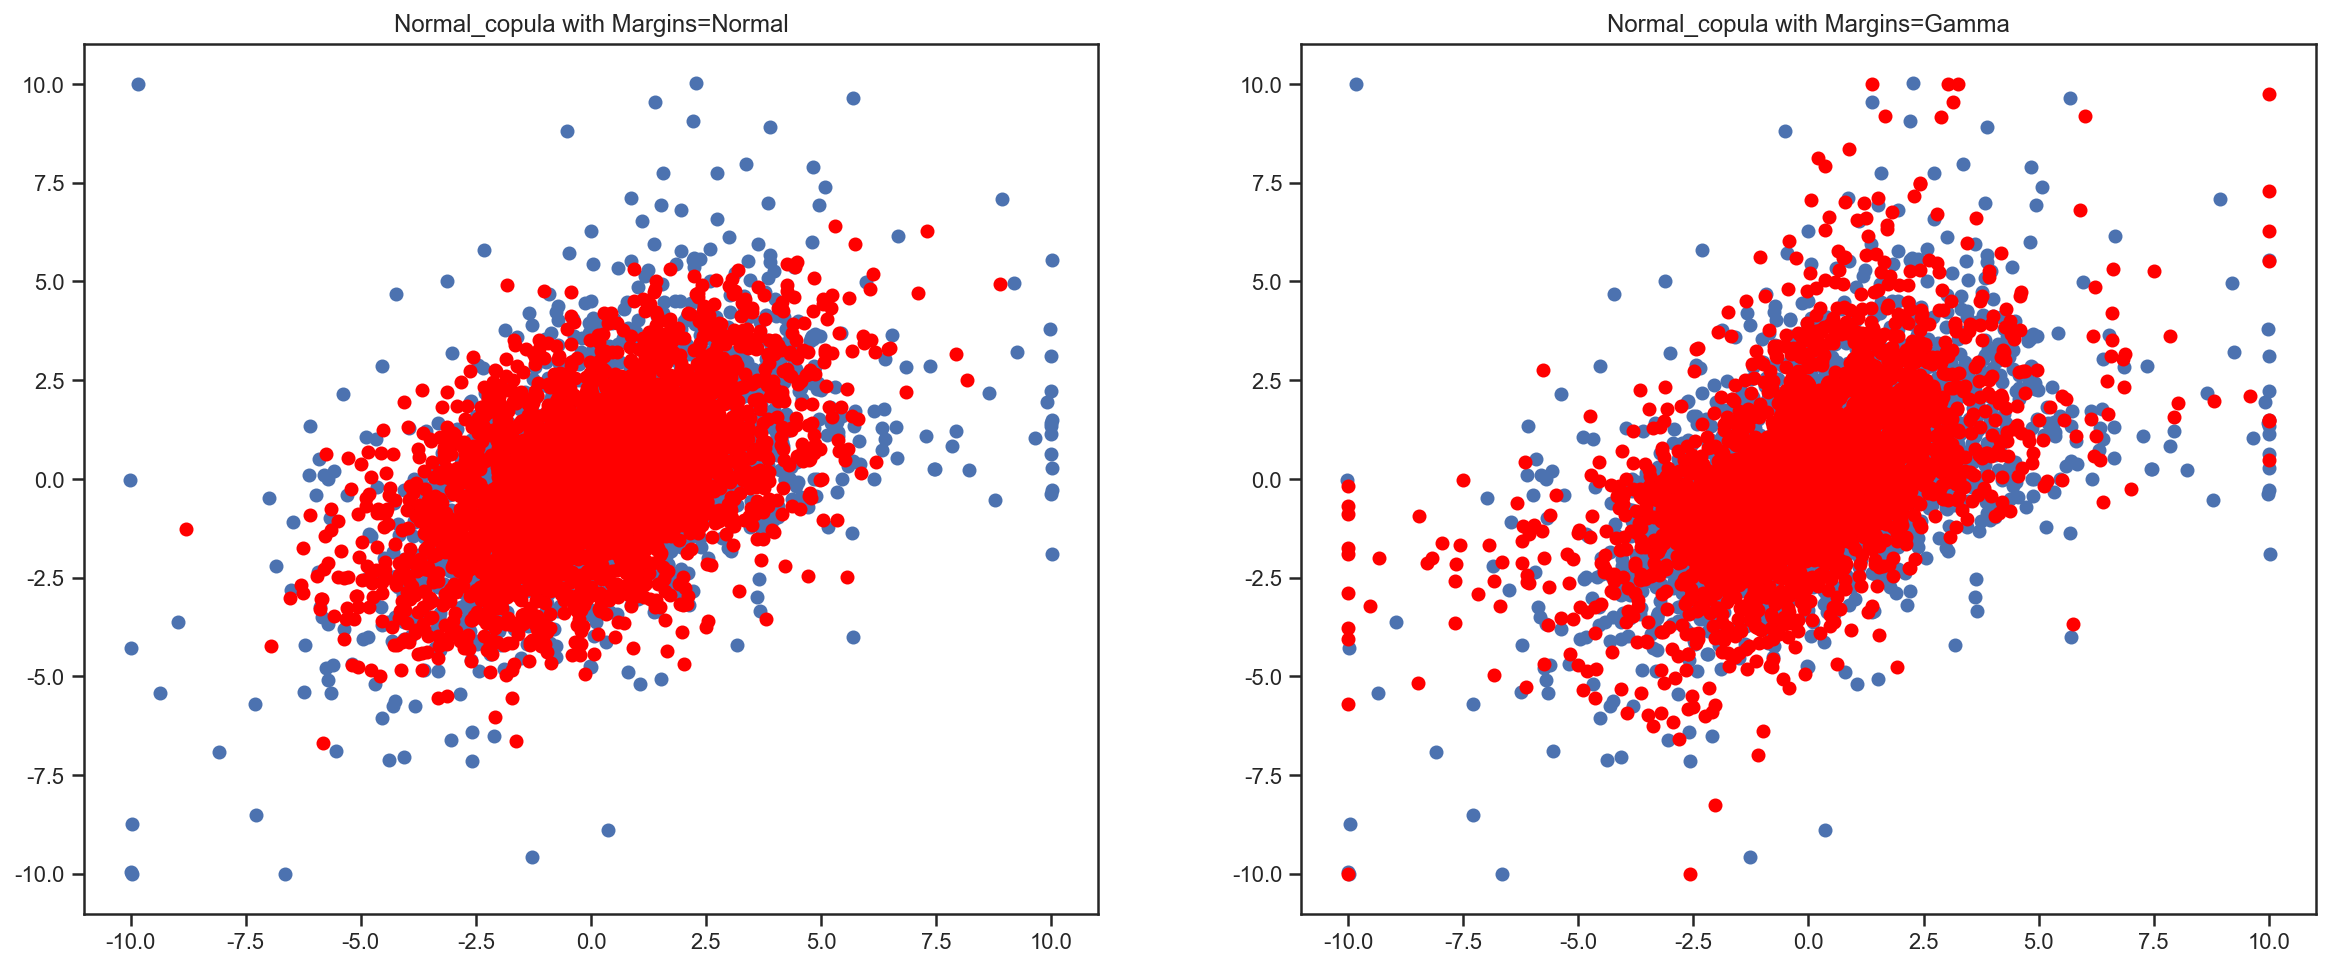
\includegraphics[scale=0.4]{figure/Copula_contrast.png}
	\caption{正态Copula下不同边缘分布的对比}
\end{figure}

\begin{algorithm}{Gaussian Copula}{}
\begin{enumerate}
	\item Sample i.i.d $(Z_1,\cdots,Z_p)$ from $N(0,1)$.
	\item Using Cholesky Decomposition to $\Sigma=A A^\prime$ and obtain $[X_1,\cdots,X_p]=[Z_1,\cdots,Z_p]A^\prime$
	\item Return $(U_1,\cdots,U_p) = (\varphi(X_1),\cdots,\varphi(X_p))$
\end{enumerate}
\end{algorithm}


\subsection{t Copula}
\begin{sdefinition}{t Copula}{}
	Let $\Theta=\left\{(\nu, \Sigma): \nu \in(1, \infty), \Sigma \in \mathbb{R}^{p \times p}\right\}$ and let $t_\nu$ be a univariate $t$ distribution with $\nu$ degrees of freedom.
The Student's $t$ copula can be written as
$$
C_{\Theta}\left(u_1, u_2, \ldots, u_m\right)=\boldsymbol{t}_{\nu, \Sigma}\left(t_\nu^{-1}\left(u_1\right), t_\nu^{-1}\left(u_2\right), \ldots, t_\nu^{-1}\left(u_m\right)\right)
$$
where $\boldsymbol{t}_{\nu, \Sigma}$ is the multivariate Student's $t$ distribution with a correlation matrix $\Sigma$ with $\nu$ degrees of freedom.
\end{sdefinition}

\begin{algorithm}{Simulate a t Copula}{}
\begin{enumerate}
	\item Generate $(Z_1,\cdots,Z_p)$ from $N_p(0,\Sigma)$.
	\item Let $(X_1,\cdots,X_p)=(\frac{Z_1}{\sqrt{\frac{S}{\nu}}},\cdots,\frac{Z_p}{\sqrt{\frac{S}{\nu}}})$ where $S\sim \chi_v$ independent of $Z_i$.
	\item Return $(U_1,\cdots,U_p)=(t_\nu(X_1),\cdots,t_\nu(X_p))$.
\end{enumerate}

\end{algorithm}






\section{Archimedean Copulas}
In practice, Archimedean copulas are popular because they allow modeling dependence in arbitrarily high dimensions with \boxred{only one parameter}, governing the strength of dependence. In addition, there exists a close-form expresssion of the relationship between this parameter and \boxred{kendall tau}.
\begin{sdefinition}{Archimedean Copula}{}
Suppose $\Omega = \{\varphi:[0,1] \to [0,\infty) | \text{$\varphi$ is a continuous,
strictly monotone decreasing,} \\ \text{, and convex function with $\varphi(1)=0$.} \}$ Let $\varphi \in \Omega$, then 
$$
C(u_1,\cdots,u_p) = \varphi^{[-1]}(\varphi(u_1)+\cdots+\varphi(u_p))
$$
is indeed a copula, where  $\varphi^{[-1]}$ is $\varphi$'s pseudo-inverse defined by
$$
\varphi^{[-1]}(t) = \varphi^{-1}(t) \chi_{[0,\varphi(0)]}(t)
$$
\end{sdefinition}



\subsection{Simple Archimedean Copula}

%\begin{tabular}{|l|c|c|c|}
%\hline Name & Clayton & Gumbel & Frank \\
%\hline Generator & $\phi(t)=\left(t^{-\theta}-1\right)$ & $\phi(t)=(-\ln t)^\theta$ & $\phi(t)=-\ln t \frac{e^{-\theta t}-1}{e^{-\theta}-1}$ \\
%\hline Inverse Generator & $\phi^{-1}(s)=(1+s)^{-\frac{1}{\theta}}$ & $\left.\phi^{-1}(s)=e^{-s^{\frac{1}{\theta}}}\right)$ & $\phi^{-1}(s)=-\frac{1}{\theta} \ln \left[1-e^{-s}(1-\right.$ \\
%\hline Parameter & $\theta>0$ & $\theta \geq 1$ & $\theta \in \mathbb{R} /\{0\}$ \\
%\hline Y-Distribution & $G a m m a\left(\frac{1}{\theta}, 1\right)$ & $\alpha=\frac{1}{\theta}, \beta=1, \gamma=\left(\cos \left(\frac{\pi}{2 \theta}\right)\right)^\theta, \delta=0$ & Logarithmic series on $\mathbb{N}^{+}$ with $\alpha=\left(1-e^{-\theta}\right)$ \\
%\hline Density of Y & $\frac{1}{\Gamma\left(\frac{1}{\theta}\right)} e^{-y} y \frac{(1-\theta)}{\theta}$ & Stable $(\alpha, \beta, \gamma, \delta)$ & $\mathrm{P}[Y=k]=\frac{-1}{\ln (1-\alpha)} \frac{\alpha^k}{k}$ \\
%\hline
%\end{tabular}


\begin{table}[htb]
\centering
\rowcolors{2}{my-red}{}
\resizebox{1.1\columnwidth}{!}{
\begin{tabular}{c c c c c}
\rowcolor{my-darkred}
 \bfw{Name of copula}  & \bfw{ Bivariate copula $C_\theta(u, v)$} & \bfw{parameter $\theta$} & \bfw{generator $\psi_\theta(t)$} & \bfw{ generator inverse $\psi_\theta^{-1}(t)$} \\
\hline
Ali-Mikhail-Haq ${ }$ & $\frac{u v}{1-\theta(1-u)(1-v)}$ & $\theta \in[-1,1]$ & $\log \left[\frac{1-\theta(1-t)}{t}\right]$ & $\frac{1-\theta}{\exp (t)-\theta}$ \\
 Clayton  & {$\left[\max \left\{u^{-\theta}+v^{-\theta}-1 ; 0\right\}\right]^{-1 / \theta}$} & $\theta \in[-1, \infty) \backslash\{0\}$ & $\frac{1}{\theta}\left(t^{-\theta}-1\right)$ & $(1+\theta t)^{-1 / \theta}$ \\
Frank & $-\frac{1}{\theta} \log \left[1+\frac{(\exp (-\theta u)-1)(\exp (-\theta v)-1)}{\exp (-\theta)-1}\right]$ & $\theta \in \mathbb{R} \backslash\{0\}$ & $-\log \left(\frac{\exp (-\theta t)-1}{\exp (-\theta)-1}\right)$ & $-\frac{1}{\theta} \log (1+\exp (-t)(\exp (-\theta)-1))$ \\
Gumbel & $\exp \left[-\left((-\log (u))^\theta+(-\log (v))^\theta\right)^{1 / \theta}\right]$ & $\theta \in[1, \infty)$ & $(-\log (t))^\theta$ & $\exp \left(-t^{1 / \theta}\right)$ \\
 Independence & $u v$ & & $-\log (t)$ & $\exp (-t)$ \\
 Joe & $1-\left[(1-u)^\theta+(1-v)^\theta-(1-u)^\theta(1-v)^\theta\right]^{1 / \theta}$ & $\theta \in[1, \infty)$ & $-\log \left(1-(1-t)^\theta\right)$ & $1-(1-\exp (-t))^{1 / \theta}$ \\
 
\end{tabular}
}
\caption{Archimedean Generator}
\end{table}

\begin{figure}[htb]
	\centering
	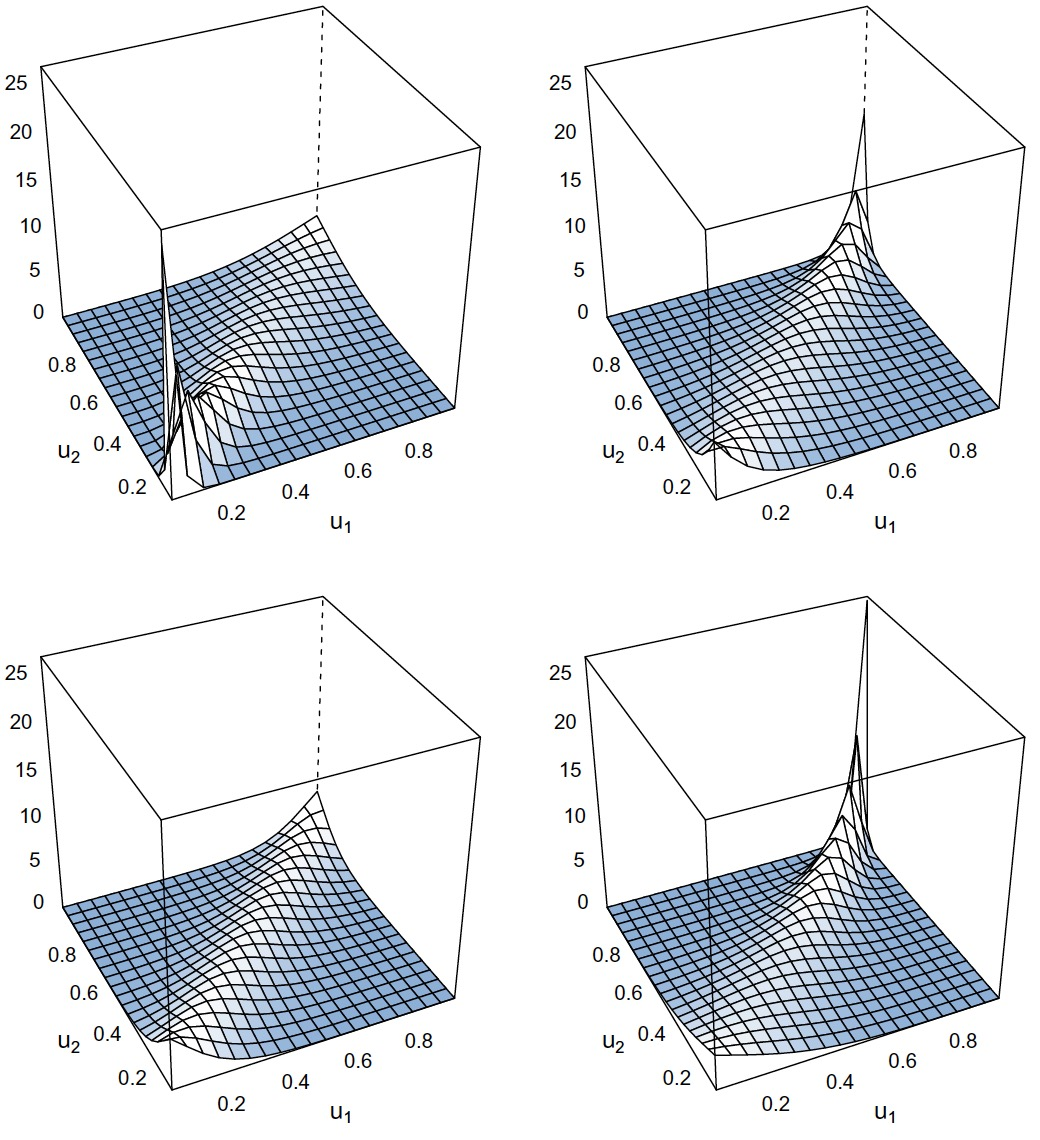
\includegraphics[scale=0.3]{figure/Archimedean.jpeg}
	\caption{Top left: Clayton, top right: Gumbel, bottom left: Frank, bottom right: Joe.}
\end{figure}


\subsection{Laplace-Lebesgue-Stieltjes Transform}
\begin{sdefinition}{Laplace-Stieltjes Transform}{}
Suppose $F:[0,\infty)\to[0,1]$ is increasing and right continuous, then the Laplace-Stielftjes Transform of $F$ is defined by 
$$
LS(F): s\mapsto \int_{\R^+} e^{-sx}\D F(x).
$$
Clearly, $LS(F): [0,\infty) \to [0,1]$ is a decreasing function with $LS(F)(0)=1$ and thus an inverse of a Archimedean Generator.
\end{sdefinition}
 
\subsection{Nested Archimedean Copula}

\subsection{Simulations}
\begin{algorithm}{Marshall and Olkin}{}
\begin{enumerate}
	\item Sample $V$ from $F = LS^{-1}(\psi^{-1})$
	\item Sample i.i.d $E_1,\cdots, E_p$ from $Exp(1)$, independent of $V$.
	\item Return $U = (\psi^{-1}(\frac{E_1}{V}),\cdots,\psi^{-1}(\frac{E_p}{V}))$
\end{enumerate} 
	
\end{algorithm}

%\bibliographystyle{siam}
%\bibliography{ref.bib}
%\printbibliography[heading = bibintoc]

\section{Applications in Assurance}
\section{Applications in Derivatives}


\end{document}